\documentclass[10pt,a4paper]{article}

\usepackage[utf8]{inputenc}
\usepackage[margin=1.2in]{geometry}
\usepackage[french]{babel}
\usepackage{amsmath}
\usepackage{amsfonts}
\usepackage{graphicx}
\usepackage{hyperref}
\usepackage[nottoc, notlof, notlot]{tocbibind}
\hypersetup{colorlinks=true,citecolor=black,filecolor=black,linkcolor=black,urlcolor=black}
\setlength{\parindent}{0.6cm} 
\setlength{\parskip}{0.10cm}
\usepackage[automark]{scrpage2}
\usepackage{color, colortbl}
\usepackage[table]{xcolor}
\usepackage{hyperref}
\usepackage{listings}
\usepackage{xcolor}


\pagestyle{scrheadings}

\ihead[]{Équipe Navigation}
\ohead[]{Plan de Développement Qualité}



\begin{document}
\pagestyle {plain}

\begin{titlepage}


\newcommand{\HRule}{\rule{\linewidth}{0.5mm}} 

\center

\textsc{\Large Université Paul Sabatier}\\[1cm] 

\includegraphics[scale=0.3]{figures/UPS.jpg}\\[0.6cm] 


\textsc{Master Intelligence Artificielle et \\ 
Reconnaissance des Formes \\ Master Robotique : Décision et Commande}\\[3cm] 

\HRule \\[0.4cm]
{ \huge \bfseries Manuel développeur}\\[0.4cm] 
\LARGE Navigation Autonome de Robot Mobile

\HRule \\[1.5cm]
 

\begin{minipage}{0.4\textwidth}
\begin{flushleft} \large
\emph{Auteurs:}\\
\href{mailto:thibaut.aghnatios@laposte.net}{Thibaut \textsc{Aghnatios} }  \\
\href{mailto:bouchetmarinee@gmail.com}{Marine \textsc{Bouchet} } \\
\href{mailto:bruno.dato.meneses@gmail.com}{Bruno \textsc{Dato} } \\
\href{mailto:klempka.tristan@gmail.com}{Tristan \textsc{Klempka} } \\
\href{mailto:lagoute.31@gmail.com}{Thibault \textsc{Lagoute} }  
\end{flushleft}
\end{minipage}
~
\begin{minipage}{0.4\textwidth}
\begin{flushright} \large
\emph{Tuteurs:} \\
\href{mailto:lerasle@laas.fr}{Frédéric \textsc{Lerasle}}\\
\href{mailto:michael.lauer@laas.fr}{Michaël \textsc{Lauer}} \\
\href{mailto:taix@laas.f}{Michel \textsc{Taix}}
\end{flushright}
\end{minipage}\\[5cm]

\large 13 mars 2017
 

\end{titlepage}

\newpage


\subsection*{Suivi du document}

\begin{center}
    \begin{tabular}{| l | l | l | l | l |}
    \hline
     \rowcolor{gray} Nom du document & Version Majeure & Version Majeure & Date de création & Dernière version \\ \hline
    Rapport & A & 0 & 13/03/2017 & 13/03/2017 \\ \hline
    \end{tabular}
\end{center}


\subsection*{Auteurs du document}

\begin{center}
    \begin{tabular}{| l | l | l | l |}
    \hline
    \rowcolor{gray} Rédaction & Intégration & Relecture & Validation Interne \\ \hline
    Equipe & ?? & ?? & ?? \\ \hline

    \end{tabular}
\end{center}

\subsection*{Validation du document}

\begin{center}
    \begin{tabular}{| l | l | l | l |}
    \hline
     \rowcolor{gray} Validation & Nom & Date & Visa \\ \hline
    & & & \\
     \hline
    \end{tabular}
\end{center}

\subsection*{Liste de diffusion}

Le rapport du projet est diffusé à l'ensemble des clients et des intervenants externes aux projets.

\subsection*{Historiques de révision}

\begin{center}
    \begin{tabular}{| l | l | l | l |}
    \hline
     \rowcolor{gray} Version & Modification apportée & Auteur & Date \\ \hline
    A.0 & Création du document & Bruno Dato & 13/03/2017\\ \hline
     
    \end{tabular}
\end{center}

\newpage
\tableofcontents
\newpage
	

\section{Présentation du projet}
\label{sec:presentation}

\subsection{Contexte}

\subsection{Problématiques}

\newpage
\section{Recherche balle}
\label{sec:recherche_balle}

\newpage
\section{Navigation avec amers 2D dans un environnement connu}
\label{sec:navigation_avec_amers_2D_dans_un_environnement_connu}

\subsection{Solution mise en place}
\label{sec:solution_mise_en_place}

\subsection{Commande haut niveau}
\label{sec:commande_haut_niveau}

\subsection{Détection et localisation}
\label{sec:detection_et_localisation}




\subsubsection{Détection}
\label{sec:detection}

\subsubsection*{Utilisation}

Nous détaillons ici les étapes nécessaires afin d'utiliser le noeud de détection. Ce noeud est lancé indépendamment des autres noeuds du système. 
Le fichier ROS de launch permet de lancer le noeud.\\
\textit{roslaunch localisation.launch}\\

Ce fichier configure et lance la détection d'amer de type AR code à l'aide d'une bibliothèque spécialisée couplée à un noeud ROS. 
Plusieurs paramètres dans ce fichier peuvent être configurés.
\begin{itemize}
\item $marker\_size$ : Largueur (cm) des marqueurs AR utilisés
\item $cam\_image\_topic$ : Topic ROS du flux d'images de la caméra.
\item $cam\_info\_topic$ : Topic ROS des infos propres à la caméra. C'est ici que les données de calibrage sont récupérées.
\item $output\_frame$ : Repère dans lequel sera exprimé le résultat de la détection.\\
\end{itemize}
Des paramètres supplémentaires se trouvent dans le fichier $localication\_node.cpp$. Le changement de ces paramètre nécessite une compilation du noeud ROS.
\begin{itemize}
\item $DEBUG$ : Active ou non les sorties de debug. Si cette option est activée, les transformations intermediaires sont publiées.
\item $TIMEOUT\_AR\_DETEC$ : Temps d'attente maximum pour la reception d'un marqueur. Ce paramètre est utile lors de l'utilisation en réseau. La latence provoque des retards dans la publication des transformées. Il est donc nécessaire de donner une marge de temps au système. Lors de l'utilisation en mode local cette valeur peut \^etre faible.
\item $NB\_MARKER$ : Nombre de marqueurs total dans la scène.\\
\end{itemize}

Une fois le lancement effectué, l'utilisateur peut observé les comportement de ce noeud avec des sorties console.
\begin{itemize}
\item $GLOBAL\_SEARCH$ : La recherche de marqueur a été demandée.
\item $ MARKER DETECTED: ID\_MARKER\_DETECTED$ : Identifiant du marqueur détecté.
\item $LOOKING FOR TF: tf$ :Nom de la transformée attendue.\\
\end{itemize}

\textit{Remarque} : Les performances de la détection des marqueurs reposent sur une bonne calibration de la caméra.






CALIBRAGE 

Pour la détection, nous utilisons la librairie $ar\_track\_alvar$ qui utilise des marqueurs AR tags.   
Cette librairie permet de détecter et de suivre ces markers en utilisant la [?]. Elle retourne l'identifiant, la position et l'orientation du marker dans la position de la $/camera\_rgb\_optical\_frame$, dans notre cas. La librairie fournie 55 AR tags et la possibilité d'entendre cette liste facilement. Dans notre cas, nous utilisons uniquement le noeud qui ne permet de lire plusieurs AR tags à la fois dans la même capture du flux vidéos. 

\lstset{language=XML}
\begin{description}
\item [Mise en place physique] : \\
 On a utilisé des AR tags de $16 \times 16$ cm. On place leur milieu à 31 cm du sol.
\item [Initialisation] : \\ Le nœud $ar\_track\_alvar$ s'initialise dans $localisation.launch$ avec les paramètres suivant : 
\begin{lstlisting}
<arg name="marker_size" default="16" />
<arg name="max_new_marker_error" default="0.08" />
<arg name="max_track_error" default="0.2" />

<arg name="cam_image_topic" 
	default="/camera/depth_registered/points" />
<arg name="cam_info_topic" 		
	default="/camera/depth_registered/camera_info" />
<arg name="output_frame" default="/camera_rgb_optical_frame" />
\end{lstlisting}

\item [Lecture du contenu [?]] : \\
	On peut écouter les ar\_track\_alvar\_msgs::AlvarMarkers que publie le nœud avec la commande : 
	\begin{lstlisting} 
	rostopic echo /ar_marker_pose
	\end{lstlisting}
\item [Performances et évolutions] : \\
	L'orientation du markeur trouvé par $ar\_track\_alvar$ doit être : $\vec{z}$ la normale et $\vec{x}$ vers le haut. Il arrive, pour des problèmes inconnus (le réseau ?) que ce repère ne soit pas correctement capturé, avec par exemple, $\vec{y}$ vers le haut. Le robot, à la fin de la localisation se trouve alors couché. Il faudrait alors comprendre d'où vient le problème ou, sinon, ne pas prendre en compte les orientations aberrantes. 
	La détection des marqueurs de $16 \times 16$ cm s'effectue jusqu'à 2m 25 avec une précision de 2 cm et jusqu'à 45\degres d'angle à 5\degres près. Il serait intéressant, à l'avenir, d'approfondir les résultats obtenus avec d'autres tailles si l'erreur est trop aléatoire, ou alors, intégrer un filtre de Kalman pour fusionner les données odométriques et les observations.

\end{description}


\begin{figure}
\center

\includegraphics[scale=0.6]{figures/artags.png} 
\caption{texte de la légende}	
\end{figure}


\subsubsection{Localisation}
\label{sec:localision}

\subsubsection*{Utilisation}
La node de localisation est lancé gr\^ace à un ficher ROS de launch. Cependant, contrairement au noeud de détection, ce noeud ne se lance pas indépendamment des autres. Il est lancé avec l'ensemble du système de navigation avec la commande suivante.
\textit{roslaunch navigation.launch}\\
blablalblalblallbla\\
blablalblalblallbla\\
blablalblalblallbla\\
blablalblalblallbla\\




blablalblalblallbla\\


\noindent Avant toute chose, il est important de rappeler que quelque soit la situation :
\begin{itemize}
\item $/map \rightarrow /odom \rightarrow /base\_link $ (\url{cf. http://www.ros.org/reps/rep-0105.html})
\item ATTENTION AU REPERE MAP [?]
\item /odom est le repère relatif de l'odométrie, assimilé certain, du robot et est placé au départ sur /map. Il est en quelque sorte le point de départ d'un déplacement. Etant donné que ce repère drift au cours du déplacement du robot, il peut être étonné. La localisation via un amer connu permet de placer le repère /odom au bon endroit, et de réinitialiser l'odométrie, ce qui place /base\_link au même endroit. C'est un localisation absolu.
\item chaque frame peut avoir plusieurs fils mais qu'un seul parent
\item la transformé entre deux frames est décrite par deux attributs : 
  \begin{itemize}
  \item $m\_origin$ : Vector3 de translation 
  \item $m\_basis$ : Matrix3x3 de rotation
  \end{itemize}
\end{itemize}

\begin{itemize}

\item [localisation\_node.cpp] :

Ce nœud permet d'envoyer la nouvelle localisation du robot si il détecte un marqueur. 

\noindent La recherche se déclanche uniquement quand la commande haut niveau publie un $<$std\_msgs::Empty$>$ sur le topic $/nav/HLC/askForMarker$. \\

Dans le cas ou un marqueur est visible : \\
\noindent \underline{init} 
/map $\rightarrow$ /odom $\rightarrow$ /baselink $\rightarrow$ /camera\_rgb\_frame $\rightarrow$ /camera\_rgb\_optical\_frame \\
\noindent \underline{arrivée d'un marker} 
/camera\_rgb\_optical\_frame $\rightarrow$ /ar\_marker\_0 \\
\noindent \underline{traitement} \\
\indent /baselink $\rightarrow$ /camera\_rgb\_frame $\rightarrow$ /camera\_rgb\_optical\_frame $\rightarrow$ /ar\_marker\_0 \\
\indent on sait donc /ar\_marker\_0 $\rightarrow$ /baselink 
= /marker\_0 $\rightarrow$ /baselink \\
\indent sachant /map $\rightarrow$ /marker\_0, on sait /map $\rightarrow$ /baselink = /map  $\rightarrow$ /odom \\

\noindent Cette transformation est envoyé sur $/new\_odom$ que l'on publie avec le publisher $odom\_pub$. On publie également l'id du marqueur vu sur $/nav/loca/markerSeen$ sous un $<$std\_msgs::Int16$>$. 

Dans le cas où on ne voit rien on publie : -1 \\

\item [localisation\_broadcaster\_node.cpp] :

Ce nœud permet de tout le temps broadcaster la transfom entre /map et /odom. Il souscrit à la $<$geometry\_msgs::Transform$>$ /new\_odom, qui contient la "nouvelle" position certaine du robot. Dès que celle-ci est publiée, /odom actualise sa position et on réinitialise le nav\_msgs/Odometry : il devient notre nouveau référentiel.
\end{itemize}

\begin{figure}
\center
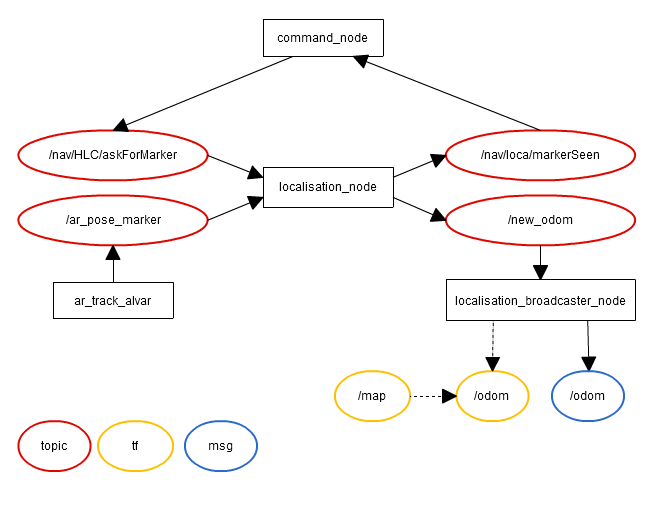
\includegraphics[scale=0.6]{figures/rqt_loca.png} 
\caption{texte de la légende}	
\end{figure}


\subsection{Commande}
\label{sec:commande}


\newpage
\section{Conclusion}
\label{sec:conclusion}

\newpage
\listoffigures
\newpage

\section*{ANNEXE}





\end{document}

